\documentclass{scrreprt}

\usepackage{aligned-overset}
\usepackage{amsmath}
\usepackage{amssymb}
\usepackage{bm}
\usepackage[shortlabels]{enumitem}
\usepackage{hyperref}
\usepackage[utf8]{inputenc}
\usepackage{mathtools}
\usepackage{physics}
\usepackage{tabularx}
\usepackage{titling}
\usepackage{fancyhdr}
\usepackage{xfrac}
\usepackage{pgfplots}

\pgfplotsset{compat = newest}
\usepgfplotslibrary{fillbetween}

\author{Albina Oscherowa \\ Lukas Kamratzki \\ Karsten Lehmann}
\date{SoSe 2021}
\title{Hausaufgabe 06 \\Analysis - Weiterführende Konzepte}

\setlength{\headheight}{26pt}
\pagestyle{fancy}
\fancyhf{}
\lhead{\thetitle}
\rhead{\theauthor}
\lfoot{\thedate}
\rfoot{Seite \thepage}

\begin{document}

\section*{Hausaufgabe 1}

Untersuchen Sie, ob die Funktion
\[
  f \colon \mathbb{R}^2 \to \mathbb{R} \text{ mit }
  f\qty(x_1, x_2) \coloneqq \sin\qty(x_1) \cdot \ln\qty(2 + \sin(x_2))
\]
auf der Menge
\[
  K \coloneqq \qty{x = \qty(x_1, x_2) \in \mathbb{R}^2 \middle| \qty(0 \leq x_1) \land \qty(2\qty(x_2 - 2)^2 + x_1 \leq 4)}
\]
Maximum und Minimum besitzt. \\

\textit{Lsg.} Aus den Beschränkungen für $x_1$ und $x_2$ folgt
\[
  0 \leq x_1 \leq 4 \text{ und } 2 - \sqrt{2} \leq x_2 \leq 2 + \sqrt{2}
\]
$\Rightarrow K \subseteq [0, 4] \times [0, 4] \Rightarrow K$ ist beschränkt.

\begin{center}
  \begin{tikzpicture}[
      declare function={
        f(\x) = 2 * (2 - (\x - 2)^2);
      }
    ]
    \begin{axis}[
      axis lines=middle,
      xlabel=$x_2$,
      xmax = 3.7,
      xmin = 0.3,
      ylabel=$x_1$,
      ymax = 4.2,
      ymin = -0.2,
      ]
      \path[name path=axisa] (axis cs:0.586,0) -- (axis cs:3.414,0);
      \addplot[
        domain = 0.586:3.414,
        very thick,
        name path = f1,
        samples = 100,
        blue,
      ] {f(x)};
      \addplot[
        fill = blue!10,
        fill opacity = .5,
      ] fill between[of = f1 and axisa];
      \node at (2,1) {$K$};
    \end{axis}
  \end{tikzpicture}
\end{center}

Die Funktionen $g_1, g_2, g_3 \colon \mathbb{R}^2 \to \mathbb{R}$ mit
$g_1\qty(x_1, x_2) = x_1$, $g_2\qty(x_1, x_2) = x_2$ und
$g_2\qty(x_1, x_2) = 2\qty(x_2 - 2)^2 + x_1$ sind stetig.
Folglich sind die Mengen
\begin{flalign*}
  A_1 &\coloneqq g_1^{-1}([0, \infty)) = [0, \infty) \times \mathbb{R} & \\
  A_2 &\coloneqq g_2^{-1}([0, \infty)) = \mathbb{R} \times [0, \infty) & \\
  A_3 &\coloneqq g_3^{-1}((-\infty, 4]) =
  \qty{\qty(x_1, x_2) \in \mathbb{R}^2 \middle| \qty(x_1 \in \mathbb{R}) \land \qty(x_1 \leq 2\qty(2 - \qty(x_2 - 2)^2))}
\end{flalign*}
als Urbilder stetiger Funktionen abgeschlossener Mengen ebenfalls abgeschlossen.
Damit ist $K = A_1 \cap A_2 \cap A_3$ als Durchschnitt abgeschlossener Mengen
abgeschlossen $\Rightarrow K$ ist kompakt.

$f$ ist eine Komposition stetiger Funktionen
$\Rightarrow f$ ist stetig
$\Rightarrow f(K)$ ist kompakt.

Damit existieren $a, b \in K$ mit $f(a) \leq f(x) \leq f(b)$ für alle
$x \in K$.

\end{document}